
%%%%%%%%%%%%%%%%%%%%%%% file typeinst.tex %%%%%%%%%%%%%%%%%%%%%%%%%
%
% This is the LaTeX source for the instructions to authors using
% the LaTeX document class 'llncs.cls' for contributions to
% the Lecture Notes in Computer Sciences series.
% http://www.springer.com/lncs       Springer Heidelberg 2006/05/04
%
% It may be used as a template for your own input - copy it
% to a new file with a new name and use it as the basis
% for your article.
%
% NB: the document class 'llncs' has its own and detailed documentation, see
% ftp://ftp.springer.de/data/pubftp/pub/tex/latex/llncs/latex2e/llncsdoc.pdf
%
%%%%%%%%%%%%%%%%%%%%%%%%%%%%%%%%%%%%%%%%%%%%%%%%%%%%%%%%%%%%%%%%%%%


\documentclass[runningheads,a4paper]{llncs}

\usepackage{amssymb, amsmath}
\setcounter{tocdepth}{3}
\usepackage{graphicx}

\usepackage{url}
\urldef{\mailsa}\path|9erthaion6@gmail.com, zaxarovyn@rambler.ru|
\newcommand{\keywords}[1]{\par\addvspace\baselineskip
\noindent\keywordname\enspace\ignorespaces#1}

\begin{document}

\mainmatter  % start of an individual contribution

% first the title is needed
\title{Numerical simulation of the dynamics of the artificial heart valve}

% a short form should be given in case it is too long for the running head

% the name(s) of the author(s) follow(s) next
%
% NB: Chinese authors should write their first names(s) in front of
% their surnames. This ensures that the names appear correctly in
% the running heads and the author index.
%
\author{D.A. Dolgov \and Y.N. Zakharov}
%
\authorrunning{CITech-2015, Almaty, Kazakhstan, 2015 September 24-27}
% (feature abused for this document to repeat the title also on left hand pages)

% the affiliations are given next; don't give your e-mail address
% unless you accept that it will be published
\institute{Kemerovo State University,\\
Kemerovo, Russia\\
\mailsa}

%
% NB: a more complex sample for affiliations and the mapping to the
% corresponding authors can be found in the file "llncs.dem"
% (search for the string "\mainmatter" where a contribution starts).
% "llncs.dem" accompanies the document class "llncs.cls".
%

\toctitle{Lecture Notes in Computer Science}
\tocauthor{Authors' Instructions}
\maketitle


\begin{abstract}
    In this paper we consider a mathematical model for describing the dynamics
    of the artificial heart valve, which is moved by the viscous inhomogeneous
    incompressible fluid flow with variable viscosity, and also a method
    of the numerical simulation of this problem. We present the results of modeling
    for the heart valve with three leaflets.
\keywords{viscous inhomogeneous fluid, artificial heart valve, immersed boundary method}
\end{abstract}


\section{Introduction}
It is difficult to overestimate the importance of medical researches of the human blood circulatory system,
because the knowledge from this area are extremely practical and significant. Each year, approximately 250 000
procedures are performed in the world to repair or replace damaged heart valves \cite{yoganathan}, and this
value tends to increace \cite{yacoub}. The solution of scientific and technical problems of the artificial valves 
creation depends on correct understanding of the fluid flow interaction with valve leaflets. Mathematical modeling
of the dynamics of artificial heart valves allows to get more complete understanding of processes inside them and helps
to find the ways to improve their design. There are many researches devoted to the mathematical and numerical modeling
of the dynamics of the heart valve. Most of them can be divided into two large groups.

First group is related to the finite element methods (\cite{taylor}, \cite{zhang}, \cite{black}). They may well handle
the complex geometry of the heart, bu the necessity to take into account the interaction between the fluid and flexible walls
leads to permanent rebuilding of the computational grid to meet the changing geometry of the object of research.
This results to significant expenses of time and computational resourses.

In this paper we consider a second approach, which is related to the immersed boundary method (\cite{pescin_1977},
\cite{boyce_2011}, \cite{ma_x_2013}, \cite{pilhwa_2010}). It can be used for the problems with complex geometry, and it doesn't
required the grid modification.

There are various improvements of this method, because of the need to model more and more complex problems. In the research \cite{fai_2013}
a formulation of this method was proposed for the three dimensional problem of the flow of two nonmixing (separated by flexible barries)
fluids of different viscosity and density. In the papers \cite{jian}, \cite{lee} an application of this method for the two dimensional problem of
the two component fluid flow.

In this work we propose to describe the blood flow in the flexible large blood vessels and the artificial heart valve as a three dimensional
nonstationary flow of the viscout incompressible fluid with variable viscosity and density (see \cite{gummel}, \cite{geidarov},
\cite{milosevic}, \cite{dolgov}). Thus the goal of this work is to build a mathematical model and a solution method of the problem
of artificial heart leaflet dynamics inside a blood vessel in view of the inhomogeneous structure of the blood, and also about the
mixture (formed elements) motion inside vessel.

\section{Mathematical formulation of the problem}

We consider a nonstationary problem of blood flow inside vessel with valve. Blood consists of the plasma and formed elements, which are approximately
45\% of the entire volume \cite{karro}. Vessel walls and valve leaflets consists of the large number of thin collagen fibers, they are flexibe
and can change their form depending on the fluid flow. The aortic valve, which are placed at the outlet from the left ventricle to the aorta, and provide
one-way movement of the blood, can be an example of this kind of systems (see Fig. \ref{fig:aortic_valve_example}):

\begin{figure}
\centering
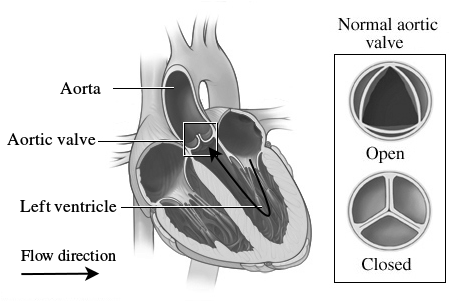
\includegraphics[height=6.2cm]{images/aorta_scheme_gray.png}
\caption{Aortic valve and its location inside heart}
\label{fig:aortic_valve_example}
\end{figure}

We model the blood as a viscous incompressible inhomogeneous two component fluid with variable viscosity, and vessel wall and valve leaflets as a
liquid impermeable surface with specified stiffness. Vessel and valve leaflets are deformed by a fluid pressure.

\begin{figure}
\centering
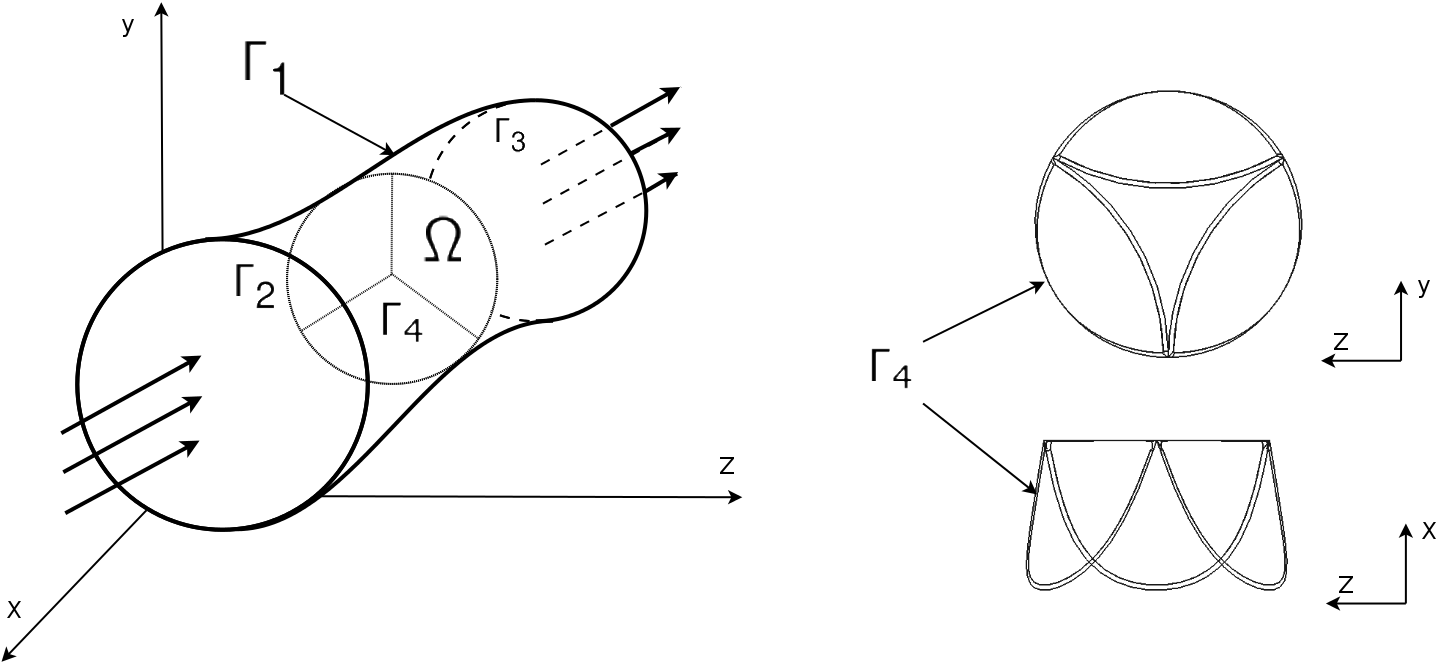
\includegraphics[width=12.5cm]{images/area_3d.png}
\caption{Scheme of the boundaries of the computational domain}
\label{fig:area_3d}
\end{figure}

Because the source of the blood motion in vessels is the pressure during the cardiac cycle, we will describe the problem of the blood flow
by the following nonstationary system of differential equations of Navier-Stokes \cite{gummel}:
\begin{gather}
    \label{eq:navier_stokes:motion}
    \frac{\partial \vec{u}}{\partial t} + (\vec{u} \cdot \nabla) \vec{u} = - \frac{1}{\rho} \nabla p + \nabla \sigma + \vec{f}\\
    \label{eq:navier_stokes:continuity}
    \frac{\partial \rho}{\partial t} + \nabla \cdot (\rho \vec{u}) = 0 
\end{gather}

with the initial and boundary conditions:
\begin{gather}
    \label{eq:navier_stokes:velocity_conditions}
    \vec{u}(\bar{x}, 0) = \vec{u}_0 \qquad \vec{u}|_{\Gamma_1, \Gamma_4} = \vec{u}_b \qquad u_{\Gamma_2, \Gamma3} = 0\\
    \label{eq:navier_stokes:pressure_conditions}
    p_{\Gamma_2} = p_{in} \qquad p_{\Gamma_3} = p_{out}
\end{gather}

where $\bar{x}=(x,y,z) \in \Omega$, $\vec{u}=(u,v,w)$ - velocity vector, $\vec{u}_b$ - velocity of the vessel wall and valve leaflet motion during the deformation,
$\rho=\rho(\bar{x}, t)$ - density, $p=p(\bar{x}, t)$ - pressure, $\sigma = \mu (\nabla \vec{u} + (\nabla \vec{u})^T)$ - viscous stress tensor,
$\mu = \mu(\bar{x}, t)$ - viscosity of fluid, $\vec{f} = \vec{f}(\bar{x}, t)$ - vector of body forces, which is futher used to determine form of the vessel and valve leaflets. 

Density $\rho$ and viscosity $\mu$ are defined by following relations \cite{gummel}:
\begin{gather}
    \label{eq:viscosity}
    \mu = c (\mu_2 - \mu_1) + \mu_1\\
    \label{eq:density}
    \rho = c (\rho_2 - \rho_1) + \rho_1
\end{gather}

where $\rho_1$, $\mu_1$ - density and viscosity if fluid (plasma), $\rho_2$, $\mu_2$ - density and viscosity of mixture (formed elements), $c$ - concentration of mixture. Concentration $c=c(\bar{x}, t)$, $c \in [0, 1]$ of mixture are determined as a solution of equation:
\begin{gather}
    \label{eq:convection}
    \frac{\partial c}{\partial t} + \vec{u} \cdot \nabla c = 0
\end{gather}

with initial conditions:
\begin{gather}
    \label{eq:convection:conditions}
    c(\bar{x}, 0) = c_0(\bar{x}), \bar{x} \in \Omega
\end{gather}

and boundary conditions at the inlet boundary:
\begin{gather}
    \label{eq:convection:conditions}
    c(\bar{x}, t)|_{\Gamma_2} = c_s(\bar{x}, t)
\end{gather}

where $c_0, c_s$ are predefined functions.

Lack of definition for one component of velocity vector at the inlet-outlet is the one of issues for computational solution of this kind of problems.
It can be solved by the using the original equations (\ref{eq:navier_stokes:motion}) - (\ref{eq:navier_stokes:pressure_conditions}) at the boundaries
$\Gamma_2$, $\Gamma_3$ for determine of missing components of the velocity vector (see details \cite{gummel}).

Motion of the vessel walls and valve leaflets is defined by forces, which returned it to the original position. Valve leaflets can be deformated much more,
than vessel walls. To describe the forces, arising due the valve deformation, we use following formula:

\begin{gather}
    \label{eq:boundary_force}
    F = \frac{\partial}{\partial s} (T \tau) + \frac{\partial^2}{\partial s^2} (E \cdot I \frac{\partial^2}{\partial s^2} X)
\end{gather}

where $\bar{q} = (q, r, s) \in \Gamma_4$, $X(\bar{q})$ - function for describing the surface of leaflets at the moment $t$, the coordinates $q, r, s$ chosen so
that the surface $X$ was presented by the large amount of parametric lines $s \rightarrow X(q^0, r^0, s)$, $T$ - tension, that arises due the stretching along $s$,
$E$ - Young's modulus, $I$ - cross-sectional moment of inertia (see \cite{boyce_2011}, \cite{pescin_2002}). Physically the formula above means,
that the valve leaflets are resist extension, compression (it's related to the first term with $T$, which is dependent on stiffness coefficient $k$),
and bending (this related to the second term, where $E$ and $I$ are referred as a stiffness coefficient $k_b$). Formula (\ref{qs:boundary_force}) allows to
take into account any changes of the valve shape.

To compture forces, arising due the deformation of the vessel, we use another formula, which allows to take into account only small changes of the shape:

\begin{gather}
    \label{eq:boundary_force_simple}
    F = k \|X - X_0\|
\end{gather}

where $\bar{q} = (q, r, s, t) \in \Gamma_1$, $X(\bar{q}, t)$, $X_0(\bar{q}, 0)$ - functions for describing the surface of vessel walls at the moment $t$ and at the initial time, $k$ - stiffness coefficient.

As shown in the works \cite{pescin_1977}, \cite{boyce_2011}, for modeling of the interaction between vessel walls, valve leaflets and the fluid flow we need
to compute the vector of body forces $f$ in the equation of Navier-Stokes, based on the force $F$, and determine current surface $X(\bar{q}, t)$ of the vessel and valve, based on the velocity vector field $\vec{u}(\bar{x}, t)$. This is done by using the following equations:
\begin{gather}
    \label{eq:interaction:velocity}
    \frac{\partial X}{\partial t}(\bar{q}, t) = \int_{\Omega} \vec{u}(\bar{x}, t) \cdot \delta (x - X(\bar{q}, t))\; dx\; dy\; dz\\
    \label{eq:interaction:force}
    \vec{f}(\bar{x}, t) = \int_{\Gamma} \vec{F}(\bar{q}, t) \cdot \delta (x - X(\bar{q}, t))\; dq\; dr\; ds
\end{gather}

where $\bar{q} = (q, r, s) \in \Gamma$ - point at the vessel wall or valve leaflet, $X = X(\bar{q}, t)$ - function for describing the surface
of vessel wall and valve leaflet at the momen $t$, $F = F(\bar{q}, t)$ - the force of resistanse to deformation,
$\vec{u}(\bar{x}, t)$ - fluid velocity vector, $\vec{f}(\bar{x}, t)$ - vector of body forces, $\delta$ - Dirac delta function.

Thus we build the model, which describes the motion of the viscous inhomogeneous incompressible fluid inside vessel with valve. In this model the fluid state
and the surface $\Gamma_1 \cup \Gamma_4$ are determined independently from each other, and the influence of the valve leaflets on the fluid is reflected by
relation (\ref{eq:interaction:force}) between the vector of body forces $\vec{f}(\bar{x}, t)$ from the equation (\ref{eq:navier_stokes:motion}) and the force of resistanse to deformation $F = F(\bar{q}, t)$ from the equations (\ref{eq:boundary_force}), (\ref{eq:boundary_force_simple}).

\section{Method of solution}

As it was mentioned before, in this work we using the immersed boundary method \cite{pescin_1977}, which are based on that when fluid flows over a body,
it exerts a normal force on the surface, and if the surface is no-slip, the fluid also exerts a shear force. The surface exerts the same force of opposite sign.
This means that fluid flow around a body can be modeled by a corresponding field of the external body forces \cite{goldstain}.

Accordingly to the immersed boundary method, we will determine the fluid flow in the parallelepiped $\tilde{\Omega}$, which contains $\Omega$.
No-splip conditions are imposed at the boundaries if $\tilde{\Omega}$.
For the computation of the fluid flow we will use rectangular uniform staggered grid $\tilde{\Omega_h}$ with grid spacing $h_x$, $h_y$, $h_z$ and 
staggered arrangement of cells, where the pressure, velocity divergence and concentration are computed at the center of cell, the velocity vector components
and vector of external forces - at the boundaries of cell. To determine the deformation of the surface $\Gamma_1 \cup \Gamma_4$ we will introduce additional
area $\tilde{\Gamma}$ with Lagrangian coordinate system, which is related to the vessel walls and valve leaflets. In the $\tilde{\Gamma}$ we will construct
a new grid $\tilde{\Gamma_h}$, which cells are corresponding to the points at the $\Gamma_1 \cup \Gamma_2$. Algorithm of solution consists of the several steps:
at the grid $\tilde{\Gamma_h}$ we will solve the problem (\ref{eq:navier_stokes:motion})-(\ref{eq:navier_stokes:pressure_conditions}); then we will solve
the convection equation (\ref{eq:convection}), i.e. determine the concentration of mixture and recalculate the density and viscosity. After it we will use
the formulas (\ref{eq:boundary_force}), (\ref{eq:boundary_force_simple}) and (\ref{eq:interaction:velocity}), (\ref{eq:interaction:force}) to determine position of
leaflets and the vessel form.

Differential equation (\ref{eq:boundary_force}), (\ref{eq:convection:conditions}) is solved by the finite difference method.
To solve (\ref{eq:boundary_force}), (\ref{eq:boundary_force_simple}) we will use the splitting on physical factors scheme \cite{belotserkovsky}:
\begin{gather}
    \label{eq:splitting:intermediate_velocity}
    \frac{u^* - u^n}{\triangle t} = - (u^n \cdot \nabla) u^* - \frac{1}{\rho} \nabla \sigma + f^n\\
    \label{eq:splitting:poisson}
    \rho \triangle p^{n+1} - \nabla \rho \cdot p^{n+1} = \frac{\rho^2 \nabla u^*}{\triangle t}\\
    \label{eq:splitting:velocity}
    \frac{u^{n+1} - u^*}{\triangle t} = - \frac{1}{\rho} \triangle p^{n+1}
\end{gather}

Computational implementation of this scheme consists of 3 stages. At the beginning the intermediate field $u^*$  is computed from the known values of velocity
from the previous time step. For this equation (\ref{eq:splitting:intermediate_velocity}) is solved by the method of stabilizing corrections \cite{yanenko}.
After it a new pressure field is determined via the computational solution of (\ref{eq:splitting:poisson}) with the biconjugate gradient method usage.
And at the last stage a final velocity vector field is calculated by the formula (\ref{eq:splitting:velocity}).

After fluid flow parameters determining it is necessary to calculate new values of density and velocity. To do that a new time step for the convection
equation (\ref{eq:convection}) must be done using the obtained values of velocity components, and the density and viscosity are recalculated
by the formulas (\ref{eq:viscosity}), (\ref{eq:density}).

Next we need to determine the deformation of vessel walls and valve leaftets under influence of fluid flow, and also the distribution of body forces $f$
in the equation of fluid motion basen on this deformation. We can calculate the deformation of vessel walls and valve leaflets at this particular fluid pressure
and the appearing resistance forces using the equations (\ref{eq:interaction:velocity}) - (\ref{eq:interaction:force}), which are numerically integrated by
the any of quadrature formulas, and equations (\ref{eq:boundary_forces}) - (\ref{eq:boundary_forces_simple}). After it we recalculate the body forces $f$
and go to the next time step.

\section{Results}

We present several results of methodical calculations for the cases of constant and variable density and viscosity, whose purpose is to demonstrate the operability
of the described method and the possibility to get with its help the patterns of  leaflet deformation and mixture distribution inside the valve.
All calculations were performed in dimensionless variables. As a vessel, in which the valve was located, a circular cylinder with length $l = 1$,
radius $r = 0.11$ and wall stiffness $k = 1 \cdot 10^3$ was used, the domain $\tilde{\Omega}$ had the spatial parameters $1.0 \times 0.5 \times 0.5$,
spatial steps $h_x = h_y = h_k = 0.01$, time step $\triangle t = 0.01$.

The dynamics of valve with three leaflets under the influence of the fluid pressure with constans density and velosity is shown in Fig. \ref{fig:valve_1}.
The pressure differential $p_{in} - p_{out}$ changes periodically from 0 to 6. Coefficient of stretching resistanse $k_b = 5 \cdot 10^3$ and coefficient of
bending resistanse $k_b = 5 \cdot 10^3$ are specified for the valve leaflets.


\begin{figure}
\centering
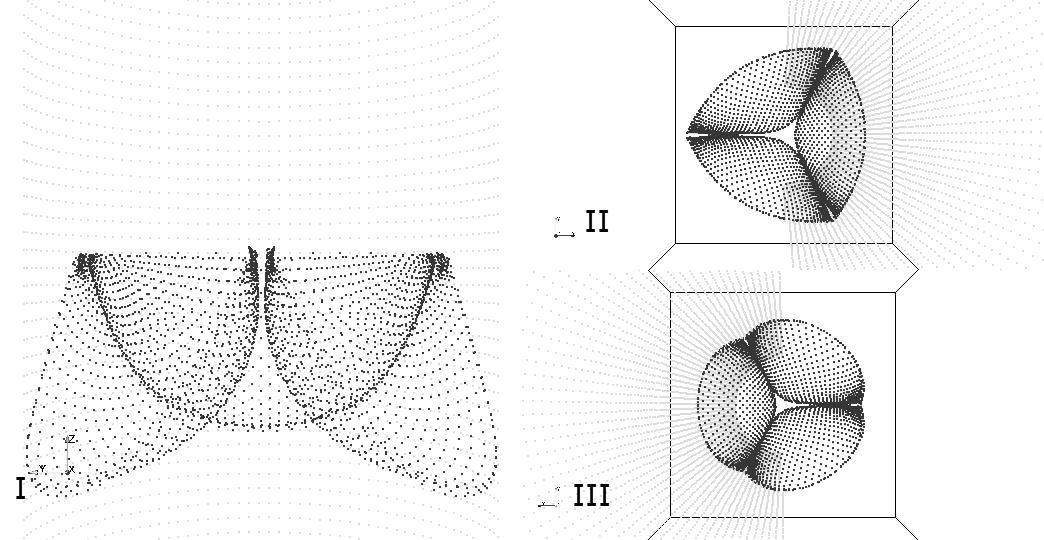
\includegraphics[height=6.2cm]{images/valve_1_gray.png}

$a$

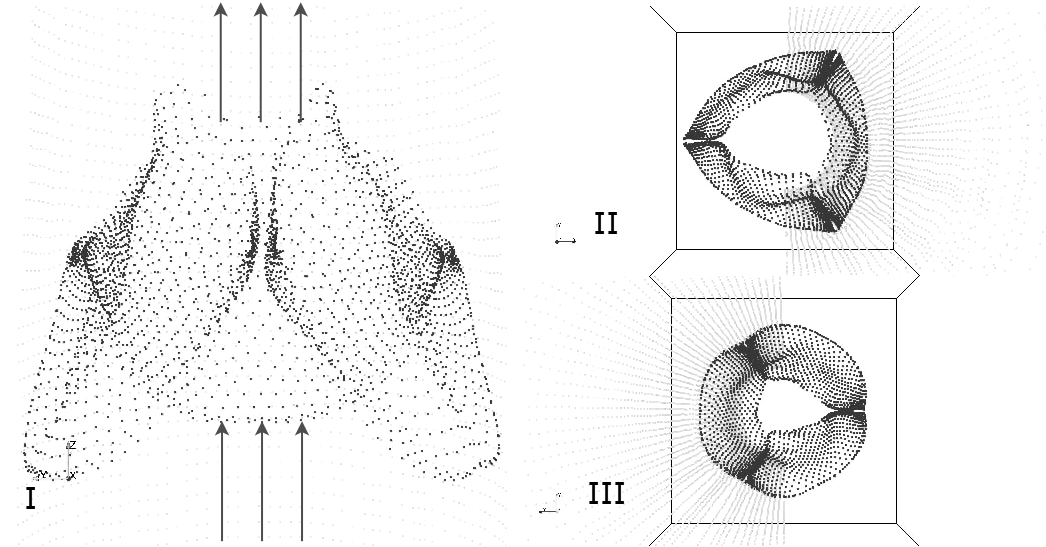
\includegraphics[height=6.2cm]{images/valve_2_gray.png}

$b$

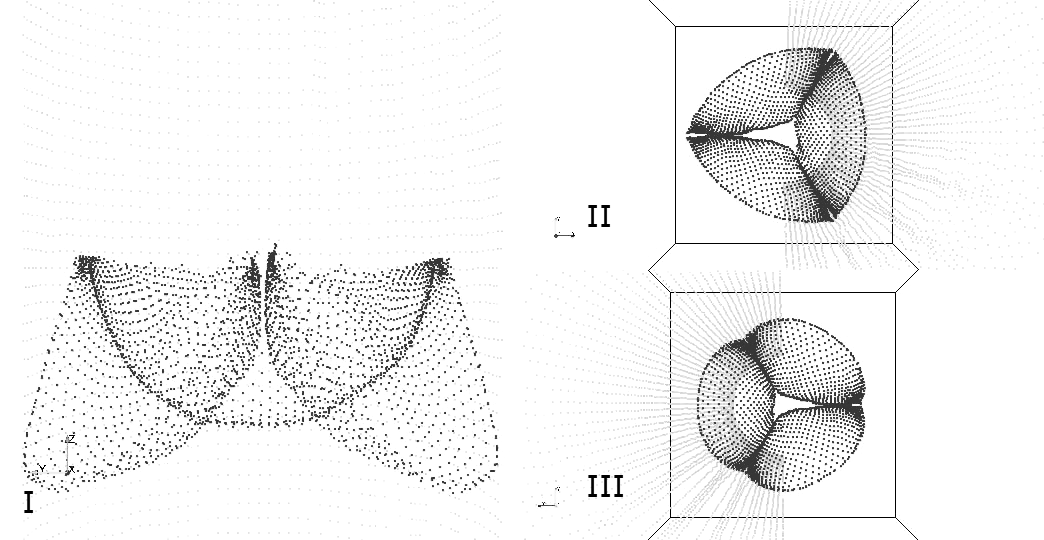
\includegraphics[height=6.2cm]{images/valve_3_gray.png}

$c$

\caption{Extended caption}
\label{fig:valve_1}
\end{figure}

\begin{figure}
\centering
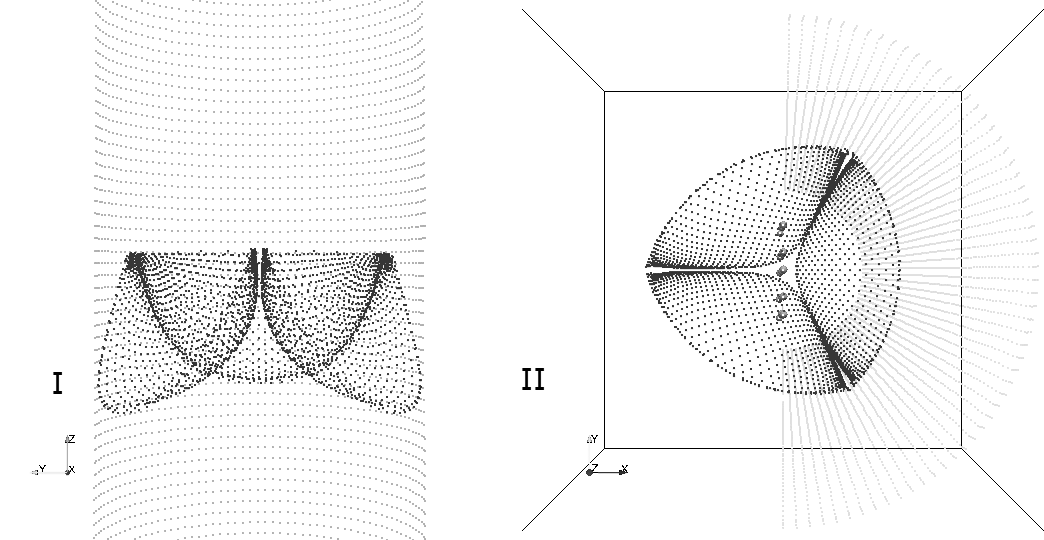
\includegraphics[height=6.2cm]{images/valve_with_particles_1_gray.png}

$a$

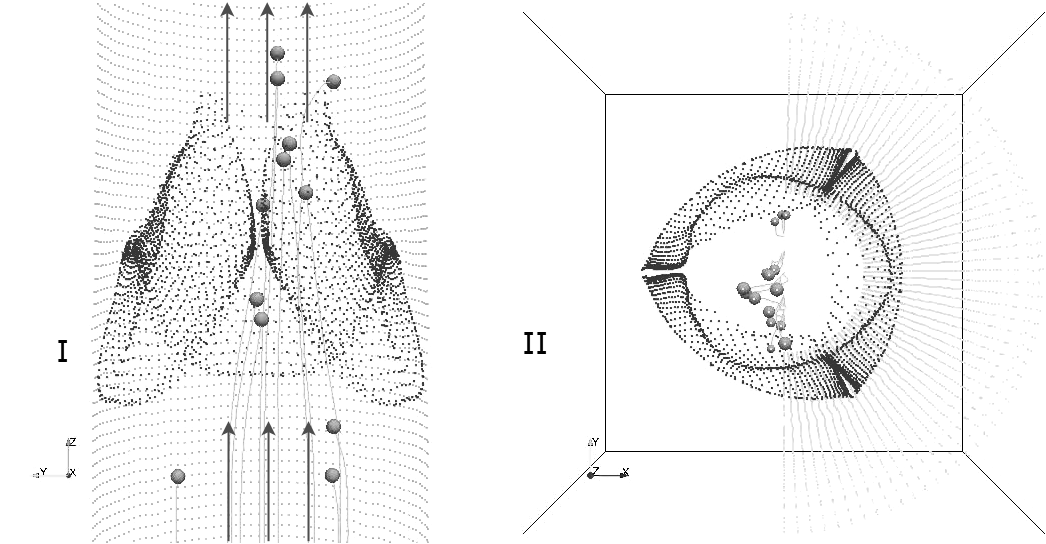
\includegraphics[height=6.2cm]{images/valve_with_particles_2_gray.png}

$b$

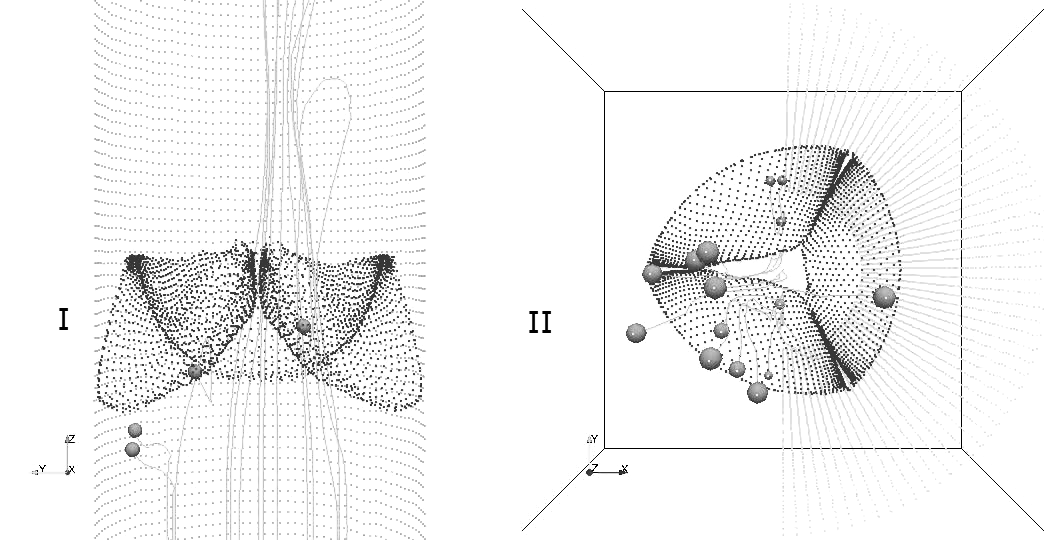
\includegraphics[height=6.2cm]{images/valve_with_particles_3_gray.png}

$c$

\caption{Scheme of the boundaries of the computational domain}
\label{fig:valve_with_particles_1}
\end{figure}

\begin{figure}
\centering
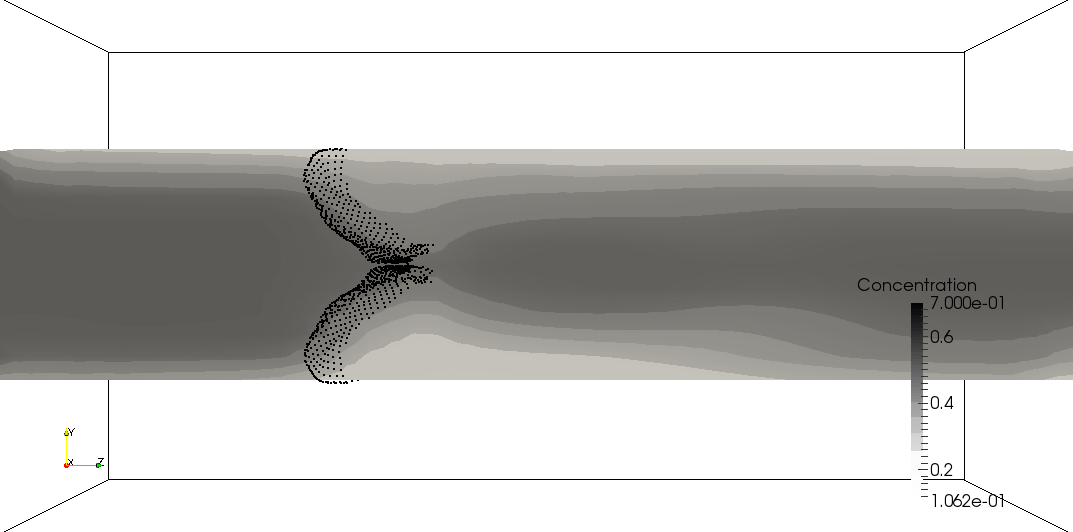
\includegraphics[height=6.2cm]{images/valves_in_mixture_gray_scale_400.png}

$a$

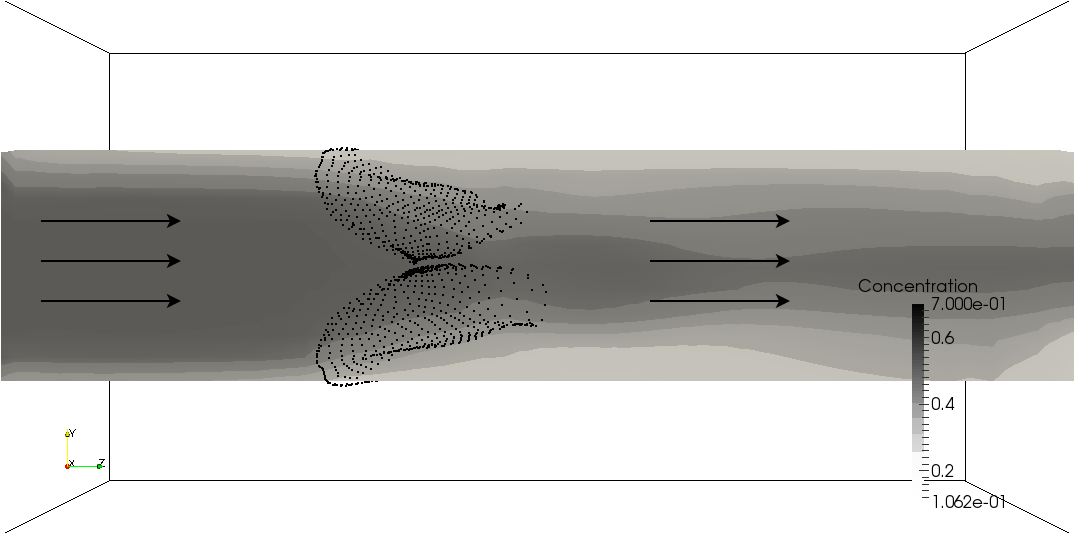
\includegraphics[height=6.2cm]{images/valves_in_mixture_gray_scale_500.png}

$b$

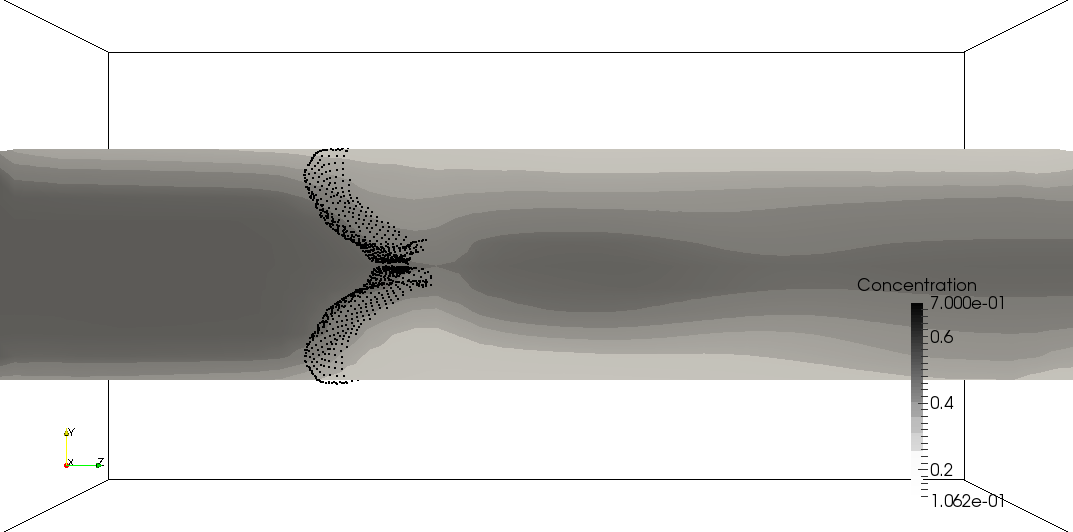
\includegraphics[height=6.2cm]{images/valves_in_mixture_gray_scale_600.png}

$c$

\caption{Scheme of the boundaries of the computational domain}
\label{fig:valve_in_mixture_1}
\end{figure}


\subsection{Citations}

For citations in the text please use
square brackets and consecutive numbers: \cite{jour}, \cite{lncschap},
\cite{proceeding1} -- provided automatically
by \LaTeX 's \verb|\cite| \dots\verb|\bibitem| mechanism.

\subsection{Page Numbering and Running Heads}

There is no need to include page numbers. If your paper title is too
long to serve as a running head, it will be shortened. Your suggestion
as to how to shorten it would be most welcome.

\section{LNCS Online}

The online version of the volume will be available in LNCS Online.
Members of institutes subscribing to the Lecture Notes in Computer
Science series have access to all the pdfs of all the online
publications. Non-subscribers can only read as far as the abstracts. If
they try to go beyond this point, they are automatically asked, whether
they would like to order the pdf, and are given instructions as to how
to do so.

Please note that, if your email address is given in your paper,
it will also be included in the meta data of the online version.

\section{BibTeX Entries}

The correct BibTeX entries for the Lecture Notes in Computer Science
volumes can be found at the following Website shortly after the
publication of the book:
\url{http://www.informatik.uni-trier.de/~ley/db/journals/lncs.html}

\subsubsection*{Acknowledgments.} The heading should be treated as a
subsubsection heading and should not be assigned a number.

\section{The References Section}\label{references}

In order to permit cross referencing within LNCS-Online, and eventually
between different publishers and their online databases, LNCS will,
from now on, be standardizing the format of the references. This new
feature will increase the visibility of publications and facilitate
academic research considerably. Please base your references on the
examples below. References that don't adhere to this style will be
reformatted by Springer. You should therefore check your references
thoroughly when you receive the final pdf of your paper.
The reference section must be complete. You may not omit references.
Instructions as to where to find a fuller version of the references are
not permissible.

We only accept references written using the latin alphabet. If the title
of the book you are referring to is in Russian or Chinese, then please write
(in Russian) or (in Chinese) at the end of the transcript or translation
of the title.

The following section shows a sample reference list with entries for
journal articles \cite{jour}, an LNCS chapter \cite{lncschap}, a book
\cite{book}, proceedings without editors \cite{proceeding1} and
\cite{proceeding2}, as well as a URL \cite{url}.
Please note that proceedings published in LNCS are not cited with their
full titles, but with their acronyms!

\begin{thebibliography}{4}

\bibitem{jour} Smith, T.F., Waterman, M.S.: Identification of Common Molecular
Subsequences. J. Mol. Biol. 147, 195--197 (1981)

\bibitem{lncschap} May, P., Ehrlich, H.C., Steinke, T.: ZIB Structure Prediction Pipeline:
Composing a Complex Biological Workflow through Web Services. In: Nagel,
W.E., Walter, W.V., Lehner, W. (eds.) Euro-Par 2006. LNCS, vol. 4128,
pp. 1148--1158. Springer, Heidelberg (2006)

\bibitem{book} Foster, I., Kesselman, C.: The Grid: Blueprint for a New Computing
Infrastructure. Morgan Kaufmann, San Francisco (1999)

\bibitem{proceeding1} Czajkowski, K., Fitzgerald, S., Foster, I., Kesselman, C.: Grid
Information Services for Distributed Resource Sharing. In: 10th IEEE
International Symposium on High Performance Distributed Computing, pp.
181--184. IEEE Press, New York (2001)

\bibitem{proceeding2} Foster, I., Kesselman, C., Nick, J., Tuecke, S.: The Physiology of the
Grid: an Open Grid Services Architecture for Distributed Systems
Integration. Technical report, Global Grid Forum (2002)

\bibitem{url} National Center for Biotechnology Information, \url{http://www.ncbi.nlm.nih.gov}

\end{thebibliography}


\section*{Appendix: Springer-Author Discount}

LNCS authors are entitled to a 33.3\% discount off all Springer
publications. Before placing an order, the author should send an email,
giving full details of his or her Springer publication,
to \url{orders-HD-individuals@springer.com} to obtain a so-called token. This token is a
number, which must be entered when placing an order via the Internet, in
order to obtain the discount.

\section{Checklist of Items to be Sent to Volume Editors}
Here is a checklist of everything the volume editor requires from you:


\begin{itemize}
\settowidth{\leftmargin}{{\Large$\square$}}\advance\leftmargin\labelsep
\itemsep8pt\relax
\renewcommand\labelitemi{{\lower1.5pt\hbox{\Large$\square$}}}

\item The final \LaTeX{} source files
\item A final PDF file
\item A copyright form, signed by one author on behalf of all of the
authors of the paper.
\item A readme giving the name and email address of the
corresponding author.
\end{itemize}
\end{document}
